\chapter{Primary Work}
\label{ch:primarywork}


This chapter will introduce the Simple Range Search and Original Range Search data structures. The Original Range Search data structure by \citet{chanetal} is a tree-like data structure with auxillary data structures. It has a space complexity of $\mathcal{O}(n)$ and a supports search queries in $\mathcal{O}(\lg\lg n + (1+k)\cdot\lg^\epsilon n)$ time, where $k$ is the amount of results reported and $\epsilon$ is an arbitrarily small constant greater than $0$.

The Simple Range Search data structure is a simplification of the Original Range Search and therefore they have the same underlying data structure. The Simple Range Search data structure has some different auxillary data structures and fewer of them. The data structure has a space complexity of $\mathcal{O}(n)$ and supports search queries in $\mathcal{O}(\lg n + (1+k)\lg^\epsilon n)$ time. Going forward,\emph{ORS} will be used as shorthand for \emph{Original Range Search} and \emph{SRS} will be used as shorthand for \emph{Simple Range Search}.


The SRS data structure has a time complexity of $\mathcal{O}(\lg n + (1+k)\cdot \lg^\epsilon n)$ which is greather than the time complexity of the ORS data structure with $\mathcal{O}(\lg \lg n + (1+k)\cdot \lg^\epsilon n)$. However, the SRS data structure is far more simple - both in code and the auxilary data structures used. The difference between the running time constant in $\mathcal{O}(\lg \lg n)$ and $\mathcal{O}(\lg n)$ is far greater than the difference between $\lg \lg n$ and $\lg n$. This makes the SRS data structure faster than the ORS data structure in practice.

\vspace{4mm}

Each section will start with a \emph{preliminaries} subsection. This subsection will describe some of the auxiliary data structures used in the section. As in Chapter~\ref{ch:relatedwork}, the main data structures in this chapter are output-sensitive and static.

\section{Simple Range Search}
\label{sect:simple}

This section will introduce the primary work of this thesis. It will show how the SRS data structure is built and how range reporting is done using the data structure. The data structure uses $\mathcal{O}(n)$ space and supports search queries in $\mathcal{O}(\lg n + (1+k)\cdot \lg^\epsilon n)$ time. This is the same space complexity as the kd-tree. The query time is different in that $\mathcal{O}(\lg n)$ is smaller than $\mathcal{O}(\sqrt{n})$, but there is a cost of $\mathcal{O}(\lg^\epsilon n)$ per point reported. 

The SRS data structure relies heavily on the \emph{ball-inheritance} data structure. The ball-inheritance structure is a tree with $n$ labelled balls at the root. In $\lg n$ steps it will distribute the balls from the root of the tree to $n$ leaves in the tree. Solving the ball-inheritance problem is to follow a ball from any given node to its leaf. We formally define the problem below in section \todo{ref}. Succint rank queries are an important part of data structure, playing a key role in solving the \emph{ball-inheritance problem}.


\subsection{Preliminaries}

\subsubsection{Rank Space Reduction}
Given $n$ points from a universe $U$, the rank of a given point in a sorted list of points is defined as the amount of points which preceed it in the list. Given two points $a,b \in U: a < b$ \emph{iff} $rank(a) < rank(b)$. Expanding this concept to 2 dimensions we have a set $P$ of $n$ points on a $U \times U$ grid. We compute the \emph{x-rank} $r_x$ for each point in $P$ by finding the rank of the x-coordinate among all the x-coordinates in $P$. The \emph{y-rank} $r_y$ finds the rank of y-coordinate among all of the y-coordinates in $P$. Using \emph{rank space reduction} on $P$, a new set $P^*$ is constructed where $(x,y) \in P$ is replaced by $(r_x(x), r_y(y)) \in P^*$. Given a range query $q = [x_1, x_2] \times [y_1, y_2]$, a point $(x,y) \in P$ is found within $q$ \emph{iff} $(r_x(x), r_y(y))$ is found within $q^* = [r_x(x_1), r_x(x_2)] \times [r_y(y_1), r_y(y_2)]$. Computing the set $P^*$ from $P$ using rank space reduction, $P^*$ is said to be in rank space. While the $n$ points could be represented by $\lg U$ bits in $P$, they can now be represented by $\lg n$ bits in $P^*$ with $\lg n \ll \lg U$ when $n \ll U$ which saves memory. Given $n$ points from $U$ we can translate them to rank space by inserting them in an array $A[1..n]$ and sort $A$. A point's index in $A$ is now its rank. In order to translate a search query $q = [x_1, x_2]$ to rank space, we will look up the successor of $x_1$ in $A$ and the predecessor of $x_2$ in $A$. The indices of these two points delimits the search query in rank space. The array $A$ acts as a mapping to and from rank space. \todo{rephrase} When a rank space reduction has been applied and there exists an array $A[1..n]$ mapping the elements to and from rank space, the algorithms used will only use RAM operations on integers of $\mathcal{O}(\lg n)$ bits.

\subsubsection{Predecessor search using binary search}
In order to find the rank space successor or rank space predecessor of a point, a binary search is used on a sorted array of points. This data structure uses $\mathcal{O}(n)$ space and have a query time of $\mathcal{O}(\lg n)$. By locating the first key in the array that is greater than or equal to the search query, the index of that key is the \emph{rank space successor}. Similarly, by locating the last key that is smaller in the array, the index of that key is the \emph{rank space predecessor}.



\subsubsection{Succint rank queries}
\label{sssect:succintrank}
Consider an array $A[1..n]$ with elements from some alphabet $\Sigma$. Given an index $i$ in the array, we can report how many elements in $A[1..i]$ are equal to $A[i]$. This is called a \emph{rank query}. We want to be able to compute a rank query in constant time using a data structure of $\mathcal{O}(n \lg \Sigma)$ bits. In order to do this, checkpoints are created. For each character in the alphabet $\Sigma$, the checkpoint contains the number of times that character appears in $A[1..i]$, where $i$ is the checkpoint location. Such a checkpoint takes up $\mathcal{O}(\Sigma \lg n)$ bits of space. By placing the checkpoints $\Sigma \lg n$ entries apart of each other, all of the checkpoints use $\mathcal{O}(\frac{n}{\Sigma \lg n} \cdot \Sigma \lg n) = \mathcal{O}(n)$ bits of space.

Each entry in $A$ contains a character from the alphabet $\Sigma$. At $A[i]$ we also store the amount of times the character at $A[i]$ occurs since the last checkpoint. This is a smaller number and can be stored using $\mathcal{O}(\lg (\Sigma \lg n))$ bits per entry in $A$. This is because we only need $\lg x$ bits to store a number which has a maximum value of $x-1$. This approach fits the required space bound if $\Sigma \geq \sqrt{\lg n}$ \todo{replace $\sqrt{\lg n}$ with $\lg^\epsilon n$}, because there $\Sigma$ will dominate the complexity. Hence, storing $n$ entries uses $\mathcal{O}(n\cdot\lg(\Sigma \lg n)) = \mathcal{O}(n\cdot\lg\Sigma) =  \mathcal{O}(n)$ bits \todo{Inkluderer ``per level''?}.\todo{Er det ved ``to dominate'' betyder i dette tilfælde?} Working under the word-RAM model of computation, we are able to pack the integers into words of $\lg m$ bits, where $m$ is the maximum number which needs to be stored.

For smaller alphabets, another scheme is used. Checkpoints are still stored at every $\Sigma \lg n$ positions. These are now called major checkpoints. In addition to this, minor checkpoints are added. These minor checkpoints are added at every $\lg \lg n$ positions and contain the amount of times each character is seen since the last major checkpoint. These minor checkpoints take up $\mathcal{O}(\Sigma \lg \lg n)$ bits each. $A[i]$ now stores the character from the alphabet $\Sigma$ and how many times that character occurs since the last minor checkpoint. In order to answer the rank query, a query to the last major checkpoint and the last minor checkpoint has to be made. Given that $\Sigma \lg \lg n \leq \sqrt{\lg n} \cdot \lg \lg n$, the array entries holding the amount of times $A[i]$ is seen since the last minor checkpoint fits into $\mathcal{O}(\sqrt{\lg n} \cdot \lg^2 \lg n)$ bits. Therefore it is possible to store these array entries in plain form, and with the help of a precomputed table of $n^{\mathcal{O}(1)}$ space we can answer rank queries between minor checkpoints in constant time. \todo{Plain form?} \todo{rephrase} \todo{Maybe only need large alphabet +  bit vector. Then can leave out complicated multilevel}

%\noindent \textbf{Ball Inheritance Problem.} Given a perfect binary tree with $n$ leaves, we want to distribute $n$ labelled balls which appear in an ordered list at the root to the leaves in $\lg n$ steps. \todo{Rephrase}. The list of balls at a given node will inherited by its children with each child receiving the same amount of balls. Each level of the tree contains the same amount of balls. Eventually each ball reaches a leaf of the tree and each leaf will contain exactly one ball. The identity of a given ball is a node and the index of the ball in that nodes list. The true identity, the information the ball contains, only lies in the leaf. The \emph{ball-inheritance problem} is to track a ball from a given node to a leaf and report the identity of the leaf. \\


\subsubsection{Ball Inheritance}
Consider a perfect binary tree with $n$ leaves and $n$ labelled balls at the root. The balls have been distributed from the root to the leaves in $\lg n$ steps, where each node picks one of its children to inherit a given ball. Both children of a node will receive the same amount of balls. The balls at the root are contained in an ordered list, and they will retain this order at all internal nodes. Each node contains a list of which ball goes to which child. The level of a node is defined to be the height of the node from the leaves. The root has the highest level, while each node is one level smaller than its parent. The leaves are at level $0$. Each level of the tree contains the same amount of balls, and at level $i$ each node contains $2^i$ balls. Eventually each ball reaches a leaf of the tree and each leaf will contain exactly one ball. A ball can be identified by a node and the index of the ball in the list of that node. Given the identity of a ball at any level, it is possible to follow this ball down the tree to a leaf. The goal is to track a balls inheritance from a given node to a leaf and report the identity of the leaf. We call the identity of the leaf the \emph{true identity} of a ball. \todo{Omskriv afsnit til at reflektere at boldene allerede er fordelt}


\subsection{Solving the ball-inheritance problem} 
\label{ssection:solving-ball}

Consider a perfect binary tree with $n$ leaves. At level $m$, each node contains a bit vector $A_v[1..2^m]$ used to indicate which child-node a ball is inherited by: If $A_v[i]$ is $0$ it means that the ball at index $i$ in that node was inherited by the left child and $1$ means that it was inherited by the right child. The identity of a ball is a node and an index into the list of that node. Given a node $v$ and an identity of a ball, we can now calculate the ball's identity in the child node which inherits the ball. The node can answer the query $rank_v(k) = \Sigma_{i \leq k} A_v[i]$. If a ball is inherited by the right child node its new identity at that node is $rank_v(i)$ because that is how many $1$'s that preceed it in the current node. If a ball is inherited by the left child node the new identity is then $i-rank_v(i)$. With this information it is possible to traverse down the tree following a ball from any given node to a leaf. There are $n$ balls per level stored in the bit vectors of the nodes on that level. Each level in the tree uses $\mathcal{O}(n)$ bits to store the bit vectors. This adds up to $\mathcal{O}(n \lg n)$ bits, or $\mathcal{O}(n)$ words in all. This trivial solution to the ball-inheritance problem uses $\mathcal{O}(\lg n)$ query time, given that it follows a ball $\mathcal{O}(\lg n)$ steps down to its leaf. The rank function is a constant time query ~\ref{sssect:succintrank}. \todo{Hvordan skal jeg referere til dette?}


\subsubsection{Faster Queries}
\label{ssection:fasterqueries}

A bit vector is an array with entries from the alphabet $\Sigma = \{0,1\}$, where each entry is used to indicate whether a left or right child has been chosen to inherit a given ball. By expanding the alphabet we can point to the children's children, $\Sigma = \{0,1,2,3\}$, the children's children's children, $\Sigma = \{0,1,2,3,4,5,6,7\}$, and so forth. Expanding the alphabet will use $\mathcal{O}(n \lg \Sigma)$ bits per level. Storing a pointer from level $i$ to level $i+\Delta$ increases the storage space by $\Delta$ bits per ball, but also enables the ball to be inherited by $2^\Delta$ descendants. By expanding the alphabet the query time can be lowered since it is possible to take bigger steps down the tree. Just like with a parent-to-child step, bigger steps are supported by succint rank queries. In order to determine the identity of a ball $b$ $\Sigma$ levels below, we need to know the destation node and how many balls before $b$ chose the same destation node. Using succint rank queries to determine the rank of a ball $\Sigma$ levels down is thus a constant time query.

Using this concept, we pick $B$ such that $2 \leq B \leq m$, where $m = \lg n$ is the height of the tree. All levels that are a multiple of $B^i$ expand their alphabet such that the balls can also reach $B^i$ levels down. If a target level does not exist, the ball points to its leaf. We need at most visit $B$ levels that are multiple of $B^i$ before reaching a level that is multiple of $B^{i+1}$, making it possible to jump down the tree with bigger and bigger steps.

% $\Sigma^{\lg_B \lg n}_i \frac{\lg n}{B^i} \cdot \mathcal{O}(B^i) = \mathcal{O}(\lg n \cdot \lg_B \lg n)$ 
Storing the expanded alphabets at each level that is a multiple of $B^i$ costs $B^i$ bits per ball. The total cost is then 
\begin{align*}
  \sum\limits_{i=1}^{\lg_B \lg n} \frac{\lg n}{B^i} \cdot \mathcal{O}(B^i) = \mathcal{O}(\lg n \cdot \lg_B \lg n)
\end{align*}


\noindent bits per ball, at all levels. With $n$ balls, this is $\mathcal{O}(n \lg_B \lg n)$ words of space with query time of $\mathcal{O}(B \lg_B \lg n)$. If we pick a $B \leq \lg^\epsilon n$ we can reduce $\lg_B \lg n$ to $\lg_{\lg^\epsilon n} \lg n = \frac{1}{\epsilon}$. Thus, the space complexity for the ball-inheritance data structure is $\mathcal{O}(\frac{1}{\epsilon} \cdot n) = \mathcal{O}(n)$ words of space. By picking $B = \lg^{\epsilon / 2} n \geq \lg \lg n$ we can find the upper bound on  the query time as follows:
\begin{align*}
  \mathcal{O}(B \lg_B \lg n) &= \mathcal{O}(B \lg \lg n) = \mathcal{O}(\lg^{\epsilon /2} n \cdot \lg \lg n)\\
  &= \mathcal{O}(\lg^{\epsilon / 2} n \cdot \lg^{\epsilon / 2} n) = \mathcal{O}(\lg^\epsilon n)
\end{align*}

\noindent The ball-inheritance problem can thus be solved in $\mathcal{O}(\lg^\epsilon n)$ time using $\mathcal{O}(n)$ words of space.
\todo{Det er fordi $\lg_B \lg n$ er det største $i$ som beskriver $B^i \leq \lg n$ }

\subsection{Solving range reporting}

Consider a perfect binary tree with $n$ leaves. The root contains $n$ points in $2$-d rank space. The elements in the ball-inheritance structure are points, so the words \emph{ball} and \emph{point} can be used interchangeably. The $n$ balls at the root of the tree are sorted by their y-rank. When distributing the balls for inheritance, a node will give both its children half of its balls: the lower half sorted by the x-rank to its left child and the upper half by x-rank to its right child. The order of the balls in a child node will be the same as the parent node. The actual coordinates of the balls are only stored at the leaves. This is how the ball-inheritance data structure was described in the previous section. The ball distribution has been specified. With this distribution, some facts about the tree can be stated. We know that the x-coordinates of the balls in the leaves are sorted from left to right - smallest to highest. The way the balls are distributed from the root, the x-coordinates are responsible for the inheritance path. \todo{rephrase} Because the nodes are sorted by their y-rank in the root node and that they keep this order, the balls in a node list at any given node is ordered by their y-rank. These two facts will be used to solve the range reporting.

\noindent Since the actual coordinates of the points are only stored once, this data structure uses linear space. \\

Given a range query $q = [x_1, x_2] \times [y_1, y_2]$ the rank successors of $x_1$ and $y_1$ and the rank predecessors of $x_2$ and $y_2$ are looked up. We know from section \todo{ref} that a range query can be translated to a rank space query. We call these $\hat{x}_1, \hat{y}_1, \hat{x}_2$ and $\hat{y}_2$. We now have our query $q$ in rank space: $\hat{q} = [\hat{x_1}, \hat{x_2}] \times [\hat{y_1}, \hat{y_2}]$. We use $\hat{x}_1$ and $\hat{x}_2$ to find the lowest common ancestor, $LCA(\hat{x}_1, \hat{x}_2)$. This node's subtree contains at least all the points with an x-coordinate between $x_1$ and $x_2$. \\

At the root we mark the positions of $\hat{y}_1$ and $\hat{y}_2$ on the bit vector. This range indicates which balls lie within the range of $[y_1, y_2]$. $i_v$ and $j_v$ will denote this range in the bit vector of the node $v$. When searching for points lying within this range, a node will update this range to fit its children. The updated range at the left child $l$ will be $i_l = i_v - rank_v(i_v)$ and $j_l = j_v - rank_v(j_v)$. The updated range at the right child $r$ will be $i_r = rank_v(i_v)$ and $j_r = rank_v(j_v)$. This is the same way the rank query was used in section \ref{ssection:solving-ball}. Now instead of just following a given ball, we keep track of a range of balls. This concept is seen on figure~\ref{fig:bitvectorsplit} \\

Traversing from the root to the $LCA$, this y-range will be updated accordingly. We know the positions of the leaves containing $\hat{x}_1$ and $\hat{x}_2$ so we can traverse from the $LCA$ down to each of them. Traversing to $\hat{x}_1$, the first stop is the left child of the $LCA$. From here, each time a node selects its left child as the path to $\hat{x}_1$ we know that the subtree contained in the right child only contains points with x-coordinates between $x_1$ and $x_2$. Symmetrically, the same applies when going right from the $LCA$: Each time a node selects a right child on the path to $\hat{x}_2$ the subtree contained in the left child only contains points between $x_1$ and $x_2$. Such a subtree is said to be fully contained. This concept is seen on figure \ref{fig:LCA}. \\

Each time a fully contained subtree is found, we want to follow all the balls lying in the y-range of the root of the subtree to their leaves. This is exactly what the ball-inheritance solves: We are given a list of ball identities and want to find their actualy coordinates. Finding a ball's coordinate from here takes $\mathcal{O}(\lg^\epsilon n)$ time per ball.

\begin{figure}[h]
    \centering
    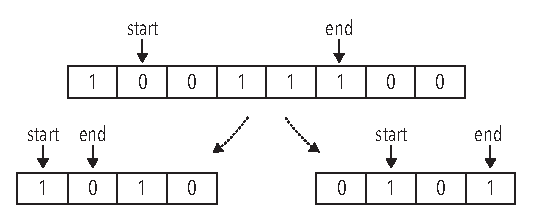
\includegraphics[width=0.95\textwidth]{pictures/bit_vector_split2.eps}
    \caption{Example of nodes inheriting their bit vector ranges from their parent.}
    \label{fig:bitvectorsplit}
\end{figure}


%The data structure is utilized as follows:
%\begin{enumerate}
%    \item Use a binary seach to find the rank space predecessors and successors of $x_1$, $y_1$, $x_2$ and $y_2$. At this point the algorithm will terminate if either rank space range is empty.
%    \item From $LCA(\hat{x}_1, \hat{x}_2)$, both $\hat{x}_1$ and $\hat{x}_2$ will be visited. The range y-rank range found in step $1$ will be updated from the root to this $LCA$ and updated from the $LCA$ to $\hat{x}_1$, $\hat{x}_2$ and all the subtrees between them.
%    \item Each time a fully included subtree is visited, we determine which balls falls within the y-range and use the ball-inheritance structure to travel to its leaf. When a leaf is visited, its actual coordinates will be reported back as a result.
%\end{enumerate}

The actual coordinates of the points are only stored at the leaves which then takes up $\mathcal{O}(n)$  words of space. The rest of the tree contains $\lg n$ levels of bit vectors of $n$ bits taking $\mathcal{O}(n \lg n)$ bits, $\mathcal{O}(n)$ words. Looking up the rank-space predecessor and successor of $x_1, x_2, y_1$ and $y_2$ using a simple binary search at the root requires $\mathcal{O}(n)$ space and $\mathcal{O}(\lg n)$ time. Summing it up, the entire data structure uses $\mathcal{O}(n)$ words of space. 

Walking from the root to the $LCA$ requires $\mathcal{O}(\lg n)$ steps. Visiting $\hat{x}_1$ and $\hat{x}_2$ requires $\mathcal{O}(\lg n)$ steps each. Visiting each of the $k$ leaves in the subtrees between $\hat{x}_1$ and $\hat{x}_2$ ,containing the points which will be reported as a result, takes $\mathcal{O}(k \cdot \lg^\epsilon n)$ time.

This adds up to $\mathcal{O}(\lg n + (1+k)\cdot\lg^\epsilon n)$ query time to report $k$ points as results. \todo{Tilføj en sætning eller to - just remake this}

\begin{figure}[h]
    \centering
    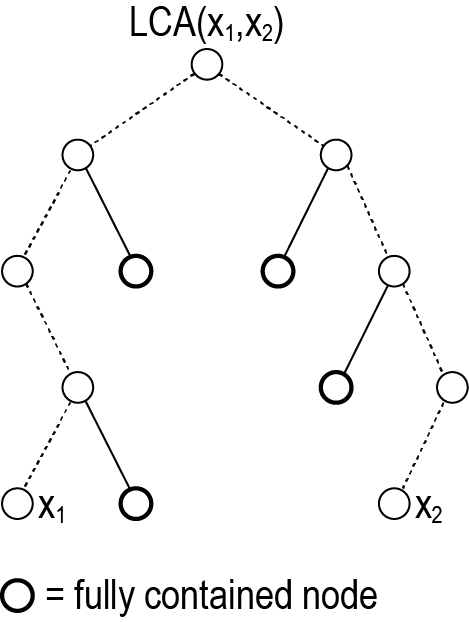
\includegraphics[width=0.6\textwidth]{pictures/LCA2.png}
    \caption{Traversing left from the LCA, each right subtree contains x-coordinates between $x_1$ and $x_2$. Traversing right from the LCA the same holds for left subtrees. Dotted line represent the path from the lowest common ancestor of $x_1$ and $x_2$ to $x_1$ and $x_2$}
    \label{fig:LCA}
\end{figure}


\section{Original Range Search}
\label{sect:original}

This section describes the ORS data structure. While the theoretical work of this thesis is a simplification of this data structure, the ORS can also be viewed as an extension of the SRS. The ORS data structure will \underline{not} be implemented, but serves as a theoretical background for the SRS. The main property the SRS and ORS share is that the underlying data structure is the ball-inheritance data structure and solving the range reporting heavily relies on solving the ball-inheritance problem.

Utilizing the ball-inheritance structure, \citet{chanetal} propose a theoretically better solution for orthogonal range search queries than the one of the Simple Range Search data structure: 
\begin{customthm}{2.1}\label{theorem21}
for any $2 \leq B \leq \lg^\epsilon n$, we can can solve $2$-d orthogonal range reporting in rank space with $\mathcal{O}(n \lg_B \lg n)$ space and $(1+k)\mathcal{O}(B \lg \lg n)$ query time.
\end{customthm}

In this section some supporting data structures will be introduced. Then we will show how the ball-inheritance is used in conjunction with these data structures to find the points within a search query $q = [x_1, x_2] \times [y_1, y_2]$.

\subsection{Preliminaries}

\subsubsection{Range minimum queries}
In order to find the smallest element in a range, a succint data structure will be used. This data structure can solve the \emph{range minimum query} problem and will be referred to as RMQ. 
Consider an array $A$ with $n$ comparable keys, this succint data structure allows finding the index of the minimum key in the subarray $A[i,j]$. \citet{fischer} introduces a data structure which solves this problem in $2n + \mathcal{O}(n)$ bits of space with constant query time. The construction requires that the array is ordered, which we will see fits into our scheme.

\subsubsection{Rank space predecessor search}
In order to look up the rank space predecessor of a given coordinate, another succint data structure will be used. This data structure has a worse space complexity than the RMQ and a bigger query time.
Given a sorted array $A[1..n]$ of $\omega$-bit integers, predecessor search queries in $\mathcal{O}(\lg \omega)$ time is supported using $\mathcal{O}(n \lg \omega)$ bits of space with \emph{oracle access} to the entries in the array. Since $\mathcal{O}(n \lg \omega)$ bits of space is not enough to store $n$ $\omega$-bit integers, the data structure will only store part of each $n$ elements and defer the look-up operation to an \emph{oracle machine}. For this purpose a Patricia trie \cite{morehaste} is used to store some parts of the $n$ $\omega$-bit integers and find which entries in the array $A$ which has to be looked up by the oracle machine. The oracle machine is some data structure that, given an index $i$, can return $A[i]$. Note that $\mathcal{O}(n)$ is less than the bits needed to store $A$. Thus, only the index of the minimum key in $A[i,j]$ can be returned, not the actual key.

\subsubsection{Finding the lowest common ancestor}
In the Simple Range Search, the lowest common ancestor of $x_1$ and $x_2$ was found by following the path from the root of the tree to both $x_1$ and $x_2$. The last node both paths shared was then the lowest common ancestor. This way of finding the lowest common ancestor takes $\mathcal{O}(\lg n)$ time which is too big for the Original Range Search.
In order to look up the lowest common ancestor of $x_1$ and $x_2$ in constant time, we are going to look at the binary representation of $x_1$ and $x_2$. First we look at $x_1 \oplus x_2$. The number of zero bits from to the start to the first one bit describes the amount of nodes the two paths have in common. We denote this number $b$. This will tell us to look on level $\lg n - b$. The number that the first $b$ bits of $x_1$ describes is the identity of the lowest common ancestor of $x_1$ and $x_2$ on level $\lg n - b$. Modern machines have an instruction for finding the most significant set bit of a number in constant time. Thus, the lowest common ancestor of $x_1$ and $x_2$ can be found in constant time.


\subsection{Solving range reporting}

With a solution to the ball-inheritance problem, \citet{chanetal} propose the following: 
\begin{customlem}{2.4}\label{lemma24}
if the ball inheritance problem can be solved with space $S$ and query time $\tau$, $2$-d range reporting can be solved with space $\mathcal{O}(S+n)$ and query time $\mathcal{O}(\lg \lg n + (1+k) \tau)$.
\end{customlem}


The ball distribution scheme of this data structure is the same as the simplified range search of section \ref{ssection:solving-ball}. Having distributed the $n$ points from the root to the leaves, additional data structures are required in order to answer the range queries. For each node in the tree that is a right child a range minimum query structure is added. The indices are the y-rank and the keys are the x-rank that the given node contains. A range maximum query structure is added to all the nodes which are left children. Each data structure uses $2n + \mathcal{O}(n)$ bits, making it $\mathcal{O}(n)$ bits per level of the tree and $\mathcal{O}(n \lg n)$ bits in all - i.e. $\mathcal{O}(n)$ words of space. \\

In order to support predecessor (and successor) search for the y-rank in the data structure, the rank space predecessor search data structure is added to the tree. This data structure works on an array of the y-ranks, which is already sorted. The points in rank space of $\mathcal{O}(\lg n)$ bits will use $\mathcal{O}(n \lg \lg n)$ bits per level, with $\omega = \lg n$, and $\mathcal{O}(n \lg n \lg \lg n)$ bits in all, which is $\mathcal{O}(n \lg \lg n)$ words. In order to reduce this to linear space we will only place this predecessor search structure at levels which are multiples of $\lg \lg n$. When using the predecessor search from the lowest common ancestor of $\hat{x}_1$ and $\hat{x}_2$, $LCA(\hat{x}_1, \hat{x}_2)$, we go up to the closest ancestor node which has a predecessor structure in order to perform the search there. Searching takes $\mathcal{O}(\lg \lg n)$ time plus $\mathcal{O}(1)$ queries to the ball-inheritance structure. The ball-inheritance structure is exactly the oracle access that the rank space predessecor search needs: At any given node the balls are sorted by their y-rank and given a the identity (the index) of a ball at that node, it can look up the y-coordinate. \todo{y-coordinate of \ldots} Using the ball-inheritance structure we walk at most $\lg \lg n$ steps down while translating the ranks of $y_1$ and $y_2$ to the right and left child of $LCA(\hat{x}_1, \hat{x}_2)$. 

The reason why this structure is necessary for the y-ranks and not the x-ranks, is because of the way the points have been distributed in the ball-inheritance tree: From left to right, the leaves have x-rank $1,2,..n$ so we can easily locate a given range in the x dimension, but in order to keep track of the y-dimensional range we need to follow the balls down the ball-inheritance structure. Adding this structure to each $\lg \lg n$ level saves us from going all the way from the root down to the $LCA$. \\

In order to use this data structure to report points in the range of $q = [x_1, x_2] \times [y_1, y_2]$ we follow these steps:
\begin{enumerate}
  \item We find the rank space successor of $x_1$ and the rank space predecessor of $x_2$. We call them $\hat{x}_1$ and $\hat{x}_2$. We use these to find the lowest common ancestor of $\hat{x}_1$ and $\hat{x}_2$, $LCA(\hat{x}_1, \hat{x}_2)$. This is the lowest node in the tree whose subtree contains at least all the points between $x_1$ and $x_2$. By knowing $\hat{x}_1$ and $\hat{x}_2$, finding the lowest common ancestor is a constant time operation.   
  \item As in step $1$ where we found the rank space of the x-coordinates, we find the rank space coordinates of the y-coordinates, $\hat{y}_1$ and $\hat{y}_2$, inside the left and right child of $LCA(\hat{x}_1, \hat{x}_2)$. We are only interested in the rank of $y_1$ and $y_2$ among the points stored in the left and right subtree of $LCA(\hat{x}_1, \hat{x}_2)$. This step is precisely what the rank space predecessor structure mentioned above supports.
  \item We now descend into the right child of $LCA(\hat{x}_1, \hat{x}_2)$ and use the range minimum query structure to the find the index $m$ (the y-rank) of the point with the smallest x-rank in the range $[\hat{y}_1, \hat{y}_2]$. The y-rank of a point at a node is exactly the identity of the ball going to the leaf storing the point. Knowing the identity of the ball we can use the ball-inheritance structure to follow the path to the leaf to find the actual x-coordinate of the point. If the x-coordinate is smaller than $x_2$ we return the point as a result and recurse into the ranges of $[\hat{y}_1, m-1]$ and $[m+1, \hat{y}_2]$ in order to find more points. Otherwise we terminate. When this is done we apply the same concept to the left child of $LCA(\hat{y}_1, \hat{x}_2)$ using the range maximum query to find points above $x_1$.
\end{enumerate}

\todo{Insert figure to conceptually show we are working our way out from the inside}

The time complexity of step $3$ depends on the use of the ball-inheritance structure. The time to traverse this structure is dependent on the improvements made in \ref{ssection:solving-ball}. An empty range will result in two queries, one query to each child of $LCA(\hat{x}_1, \hat{x}_2)$. In the worst case the amount of queries to the ball-inheritance structure will be twice the number of results reported plus one. Each time a result is found, a recursion is made to both the left and right subrange of that result. If one of the sides constantly fails to find a result, at most two queries are made for each result found. For the final result found, two ranges are recursed into which reports no results.

Conceptually, $LCA(\hat{x}_1, \hat{x}_2)$ describes a point between $x_1$ and $x_2$. Step $3$ selects points that are in the range of $[y_1, y_2]$ moving outwards from the point of $LCA(\hat{x}_1, \hat{x}_2)$, always picking the point closest to $LCA(\hat{x}_1, \hat{x}_2)$ in its decreasing y-range. \todo{rephrase}

Going back to Lemma $2.4$, we see that the time complexity fits: $\mathcal{O}(\lg \lg n)$ time is used for the predecessor search and $\mathcal{O}((1+k)\tau)$ time is used for walking from the children of the $LCA$ to the leaves solving the ball inheritance problem for the $k$ results.

\section{Summary}
\label{sect:summaryprim}

The SRS and ORS data structures both uses $\mathcal{O}(n)$ words of space. Both relies heavily on the ball-inheritance data structure in order to store and retrieve the actual coordinates of points. Both data structures supports retrieval of points through the ball-inheritance data structure in $\mathcal{O}(\lg^\epsilon n)$ time. The main difference between the SRS data structure and the ORS data structure is the rest of the query time: $\mathcal{O}(\lg n)$ for the SRS and $\mathcal{O}(\lg \lg n)$ for the ORS. The ORS data structure relies on more auxillary data structures of greater complexity than the SRS data structure. Thus, the theoretical running time of a range query to ORS is smaller than a range query to the SRS. In practise, it is safe to assume a range query to the SRS is faster than a range query to the ORS. With much more code to be executed and using more advanced auxillary data structures, the running time constant hidden in $\mathcal{O}(\lg \lg n)$ can be quite large. Also,  the factor between $\lg n$ and $\lg \lg n$ is not that big. Given a very large dataset of $2^{64}$ elements as input, $\lg 2^{64} = 64$ and $\lg \lg 2^{64} = 6$, which has a factor $\sim10$ difference. \\

The SRS and ORS data structures supports search queries in a manner similar to the range tree. A balanced binary search tree is used to locate the subtrees which is fully contained in $[x_1, x_2]$. From here the range tree uses balanced binary search trees or fractional cascading to locate which of those points are in $[y_1, y_2]$, while the SRS and ORS data structures uses the ball-inheritance structure to decode the y-ranks to actual points. \\

Both the SRS data structure and the kd-tree uses $\mathcal{O}(n)$ words of space. This is an attractive property when working on the RAM. Like all the main data structures mentioned in this thesis, the kd-tree and SRS data structure are output-sensitive. A range query to the kd-tree has a running time of $\mathcal{O}(\sqrt{n}+k)$ and a range query to the SRS data structure has a running time of $\mathcal{O}(\lg n + (1+k)\cdot\lg^\epsilon n)$. When $n$ grows, $\mathcal{O}(\sqrt{n})$ grows at a faster rate than $\mathcal{O}(\lg n)$. For each point reported as a result from a range query to the SRS data structure there is a cost of a factor $\mathcal{O}(lg^\epsilon n)$ while each point reported as a result from a range query to the kd-tree has a cost of a factor $\mathcal{O}(1)$. The $\mathcal{O}(\sqrt{n})$ running time of the range query to the kd-tree is due to a pessimistic idea that a range query will overlap, but not fully include, a lot of regions in the kd-tree. So dependent on the shape of the range query to the kd-tree, the running time can vary a lot. The $\mathcal{O}(\lg n)$ part of the range query to the SRS data structure is due to the initial binary search and to follow the path from the root of the tree to $x_1$ and $x_2$. Thus, the running time of a range query to the SRS data structure will behave more stable (fluctuate less) than the running time of a range query to the kd-tree. 


\todo{Kan man sige noget en sammenligning af de to worst-cases? At den ene er bedre end den anden og det sætter en bedre upper bound?}

Another aspect of range querying is testing for emptiness. When testing for emptiness, a range query can stop the moment a single result is found since it is a test with the binary outcome of ``yes'' or ``no''. The SRS data structure will be able to determine emptiness of a range query with no ball-inheritance queries. Hence, an emptiness query to the SRS data structure can be checked in $\mathcal{O}(\lg n)$ time. The initial binary search to find the rank space query might indicate that there are no points in $[x_1, x_2]$ or $[y_1, y_2]$. If the initial binary search does not indicate an empty range, the range query will continue normally. The moment a query to the ball-inheritance structure is made, the range is not empty and the emptiness test can report back without doing the actual ball-inheritance query. An emptiness query to the kd-tree can checked in $\mathcal{O}(\sqrt{n})$ time. The same argument as before applies: The query might overlap with a lot of regions which it does not fully contain, and within those regions none of the points are within the range. On the other hand, when a fully contained region is found the emptiness test can report back with a result. Given a range query $[x_1, x_2] \times [y_1, y_2]$, the SRS data structure will have a more stable running time for its emptiness test than the kd-tree. The running time of a query made to the kd-tree will fluctuate a lot depending on the shape of the query.

\todo{Ting du skal huske at have med i dette kapitel: Decode y-rank i stedet for at slå op i søgetræ. Range-tree imod ball-inheritance}
\todo{Balls per level vs balls per node - hvordan skal det introduceres (og hvor). Rank af bolde i node (per node)}
